\subsubsection{Анализ аналогичных разработок}


\paragraph{\href{http://www.pathguy.com/cg35.htm}{Javascript D\&D 3.5 Character Generator}}
Данное средство (рис.~\ref{ris:js_character_generator}) позволяет автоматизировать расчёт создаваемого персонажа. Предоставляется в виде интерактивной веб-страницы. Частично ведёт расчёт параметров и характеристик персонажа. После создания персонажа создаётся подходящий для печати лист.

\begin{figure}[h]
\center{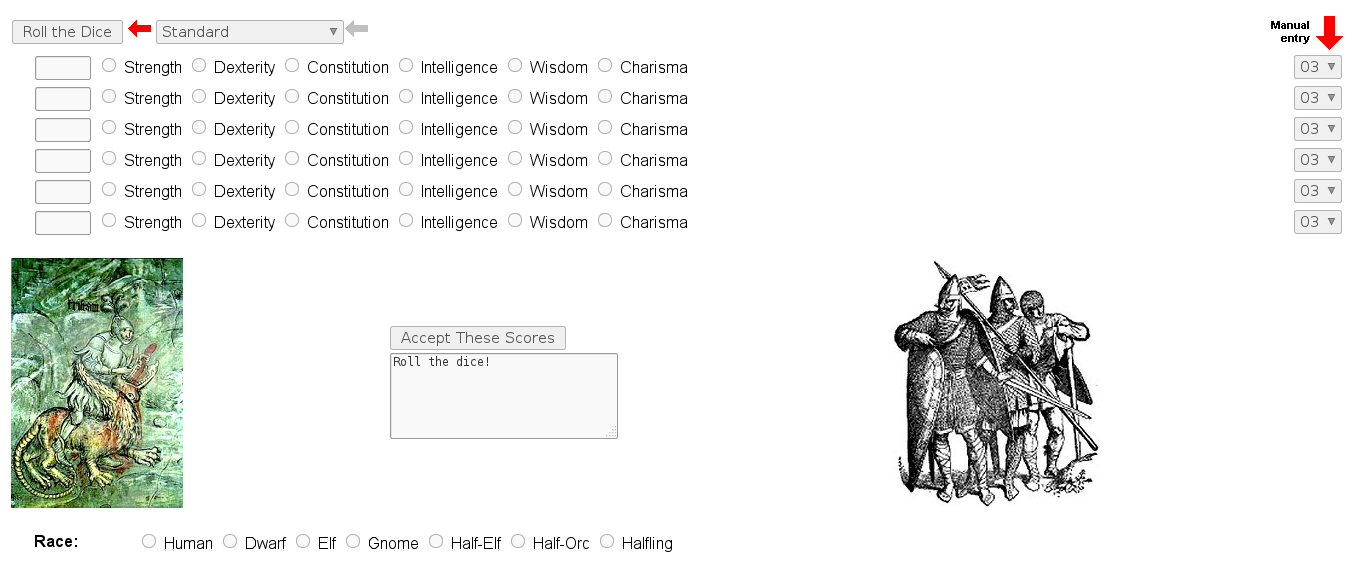
\includegraphics[width=1\linewidth]{images/similar_applications/js_character_generator}}
\caption{Внешний вид приложения <<Javascript D\&D 3.5 Character Generator>>}
\label{ris:js_character_generator}
\end{figure}


\paragraph{Dungeon\&Dragons E-Tools}
Dungeon\&Dragons E-Tools (рис.~\ref{ris:dnd_e-tools}) является десктопным приложением, которое позволяет автоматизированно создавать и генерировать персонажей, монстров, классы, расы и другой внутриигровой контент. Для работы приложения необходима ОС Windows.

\begin{figure}[h]
\center{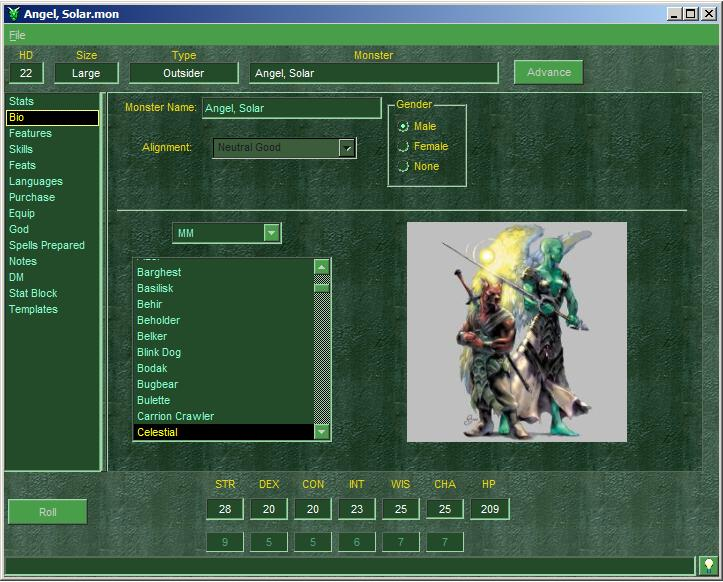
\includegraphics[width=0.8\linewidth]{images/similar_applications/dnd_e-tools}}
\caption{Внешний вид приложения <<Dungeon\&Dragons E-Tools>>}
\label{ris:dnd_e-tools}
\end{figure}


\paragraph{\href{http://www.wizards.com/dnd/Tool.aspx?x=dnd/4new/tool/adventuretools}{Dungeons \& Dragons Insider Adventure Tools}}
Данное средство автоматизации игрового процесса предоставляется официальным разработчиком игровой системы \dnd\ 4 редакции. Оно предоставляется всем подписчикам \href{http://www.wizards.com/dnd}{специализированного ресурса}.

\href{http://www.wizards.com/dnd/Tool.aspx?x=dnd/4new/tool/adventuretools}{Dungeons \& Dragons Insider Adventure Tools} (рис.~\ref{ris:dnd_insider}) предоставляет следующие возможности:
\begin{enumerate}
\item \textbf{Автоматизированное создание персонажа}. Для создания персонажа данное средство предоставляет интерактивный редактор, позволяющий частично автоматизировать расчёты при создании персонажа. Также данные редактор предоставляет возможность создания листа персонажа по его параметрам и характеристикам.
\item \textbf{Генерация способностей персонажа}. В соответствии с требованиями, которые игрок вводит в систему, данное средство способно генерировать набор характеристик.
\item \textbf{Генерация имён персонажей}.
\item \textbf{Генерация монстров}.
\item \textbf{Просмотр правил игры}.
\end{enumerate}

\begin{figure}[!h]
\center{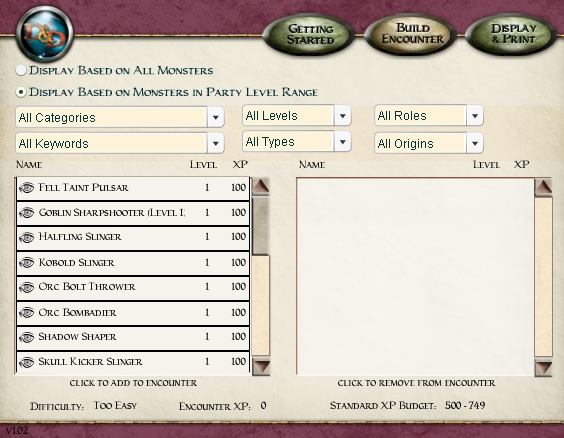
\includegraphics[width=0.8\linewidth]{images/similar_applications/dnd_insider}}
\caption{Внешний вид приложения <<Dungeons \& Dragons Insider Adventure Tools>>}
\label{ris:dnd_insider}
\end{figure}


\paragraph{D\&D 4 Android}
D\&D 4 Android (рис.~\ref{ris:dnd_4_android}) --- мобильное приложение, автоматизирующее создание персонажа. Позволяет создавать, хранить и изменять листы персонажей.

\begin{figure}[!h]
\begin{minipage}[h]{0.49\linewidth}
\flushright{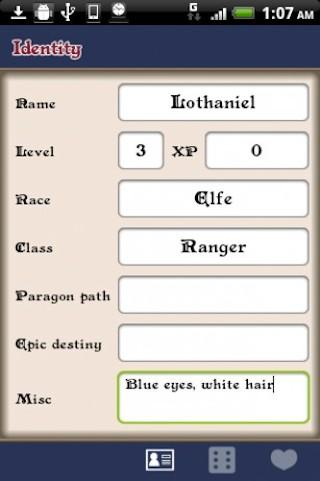
\includegraphics[width=0.65\linewidth]{images/similar_applications/dnd_4_android-1}}
\end{minipage}
\begin{minipage}[h]{0.49\linewidth}
\flushleft{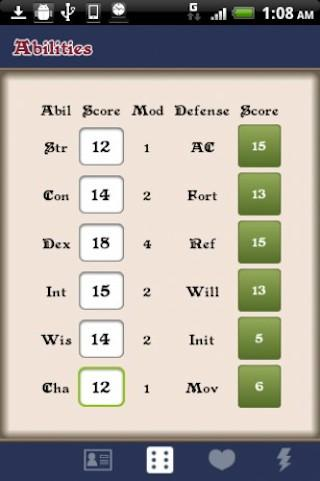
\includegraphics[width=0.65\linewidth]{images/similar_applications/dnd_4_android-2}}
\end{minipage}
\caption{Внешний вид приложения <<D\&D 4 Android>>}
\label{ris:dnd_4_android}
\end{figure}


\paragraph{DnD Buddy}
DnD Buddy (рис.~\ref{ris:dnd_buddy}) --- мобильное приложение, предлагающее следующие функции:
\begin{itemize}
\item создание персонажей;
\item импорт персонажей из D\&D Insider Adventure Tools;
\item библиотека вещей, заклинаний и пр.;
\item броски игральных костей;
\item управление сражениями;
\item создание и управление игровыми кампаниями.
\end{itemize}

\begin{figure}[!h]
\center{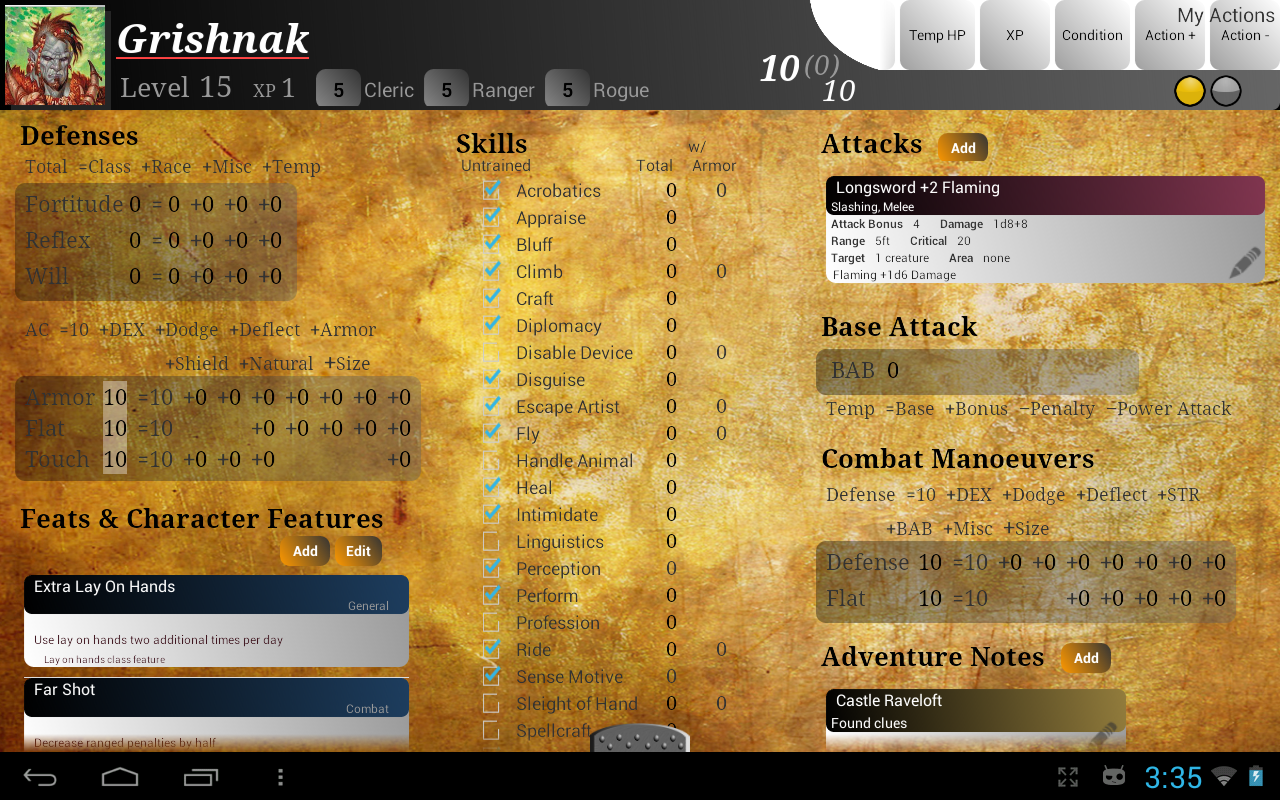
\includegraphics[width=0.8\linewidth]{images/similar_applications/dnd_buddy}}
\caption{Внешний вид приложения <<DnD Buddy>>}
\label{ris:dnd_buddy}
\end{figure}


Описанные средства имеют ряд недостатков.
\textbf{\href{http://www.pathguy.com/cg35.htm}{Javascript D\&D 3.5 Character Generator}} --- не смотря на возможность частично автоматизировать расчёт персонажа, для использования данного средства необходомо достаточно хорошо разбираться в правилах. Также данное средство не позволяет сохранять персонажей, в результате чего невозможно редактирование персонажа после получения готового листа.
Для работы \textbf{Dungeon\&Dragons E-Tools} необходима ОС Windows, что ограничивает применение этого средства для игры.
Для использования \textbf{\href{http://www.wizards.com/dnd/Tool.aspx?x=dnd/4new/tool/adventuretools}{Dungeons \& Dragons Insider Adventure Tools}} необходимо специальное дополнение для браузера от Microsoft, что нарушает принцип кроссбраузерности и ограничивает его повсеместное использование.
В \textbf{\href{http://www.wizards.com/dnd/Tool.aspx?x=dnd/4new/tool/adventuretools}{Dungeons \& Dragons Insider Adventure Tools}} и \textbf{Dungeon\&Dragons E-Tools} отсутствует какая-либо интегрированность компонент, в результате чего построение целостной системы персонажей и игр невозможно. Каждый инструмент обладает ограниченным функционалом, предоставляя минимальный необходимый набор функций.

\textbf{DnD Buddy} и \textbf{D\&D 4 Android} --- мобильные приложения для ОС Android, что ограничивает их применение только мобильными платформами.

Также стоит отметить, что \href{http://www.wizards.com/dnd/Tool.aspx?x=dnd/4new/tool/adventuretools}{Dungeons \& Dragons Insider Adventure Tools} предоставляет инструменты только для 4 редакции ролевой системы.
